\documentclass[a4paper,12pt,french]{article}
\usepackage[margin=2cm]{geometry}
\usepackage[thinfonts,latinmath]{uglix2}
\nouveaustyle


\pagestyle{empty}
\begin{document}
	\titre{Corrigé du DL1}{\premiere}{}

\exo{}\\
Soit $\lambda$ un nombre réel.\\
A, B et C sont trois points tels que $\quad AB=20\lambda +12$, $\quad BC=15(\lambda+1)\quad$ et $\quad AC=25\lambda +19$.\\
On considère le point D tel que ABCD est un parallélogramme.
\begin{enumerate}[\bfseries 1.]
	\item 	Faire un schéma et rappeler une condition nécessaire et suffisante pour qu'un parallélogramme soit un rectangle.
	\item 	Déterminer toutes les valeurs de $\lambda$ pour lesquelles ABCD est un rectangle.
	\item	 Quelle est alors la longueur BD ?\\
\end{enumerate}

\begin{exercicecorrection}
	\begin{enumerate}[\bfseries 1.]
		\item 	Un parallélogramme est un rectangle si, et seulement si, il possède un angle droit.\\
		Schéma correspondant aux données :
		\begin{center}
			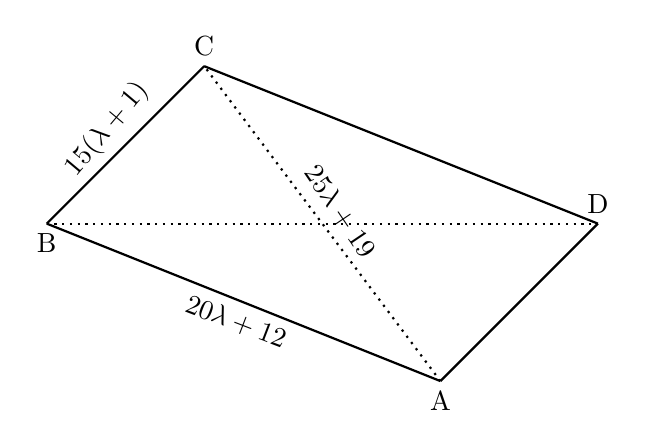
\begin{tikzpicture}[scale=1]
				\coordinate (A) at (5,0);
				\coordinate (B) at (0,2);
				\coordinate (D) at (7,2);
				\coordinate (C) at (2,4);		
				\draw[thick] 	(A) node[below]{A} -- node[midway,rotate=-21,below]{$20 \lambda + 12$} 	
				(B) node[below]{B};
				\draw[thick] (C) node[above]{C} -- 
				(D) node[above]{D};
				\draw[thick,dotted] (A) -- node[midway,rotate=-56,above]{$25 \lambda + 19$} (C);
				\draw[thick,dotted] (B) -- (D);
				\draw [thick] (B) -- node[midway,rotate=50,above]{$15(\lambda + 1)$} (C);
				\draw [thick] (A) -- (D);
			\end{tikzpicture}
		\end{center}
		\item 	 \begin{tabbing}
			ABCD est un rectangle	\= $\Leftrightarrow$ ABC est rectangle en B\\
			\>	$\Leftrightarrow AC^2=AB^2+BC^2 \quad$ \textit{d'après le théorème de Pythagore et sa réciproque}\\
			\> $\Leftrightarrow (25\lambda+19)^2=(20\lambda+12)^2+\left(15(\lambda+1)\right)^2$\\
			\> $\Leftrightarrow 625\lambda^2+950\lambda+361=400\lambda^2+480\lambda+144+225\lambda^2+450\lambda+225$\\
			\> $\Leftrightarrow 625\lambda^2+950\lambda+361=625\lambda^2+930\lambda+369$\\
			\> $\Leftrightarrow 20\lambda=8$\\
			\> $\Leftrightarrow \lambda=\dfrac{8}{20}$\\[0.5em]
			\> $\Leftrightarrow \lambda =\dfrac{2}{5}$
		\end{tabbing}	
		\item	Les diagonales d'un rectangle sont de même longueur.\\
		Donc pour $\lambda=\dfrac{2}{5}$ : $\quad BD= AC = 25\times \dfrac{2}{5}+19=29$
	\end{enumerate}
\end{exercicecorrection}


\exo{}
\begin{enumerate}[\bfseries 1.]
	\item 	Rappeler la définition d'une fonction affine.
	\item 	Démontrer la proposition suivante :\\
			\og Si $f$ est une fonction affine, alors pour tous réels $u$ et $v$, $\quad f\left(\dfrac{u+v}{2}\right)=\dfrac{f(u)+f(v)}{2}$ \fg.
	\item	Compléter la phrase suivante qui permet de reformuler cette propriété en terme de moyenne :\\
	Si $f$ est une fonction affine, alors l'image par $f$ de la moyenne de deux nombres réels est égale à \dotfill\\
\end{enumerate}

\begin{exercicecorrection}
	\begin{enumerate}[\bfseries 1.]
		\item 	$f$ est une fonction affine si :
		\begin{enumerate}[\textbullet]
			\item 	$f$ est définie sur $\R$ ;
			\item 	Il existe deux réels $m$ et $p$ tels que : \quad pour tout $x\in \R, \quad f(x)=mx+p$.
		\end{enumerate}
		\item 	Soit $f$ une fonction affine.\\
		Soient $m$ et $p$ deux réels tels que pour tout $x\in \R, \quad f(x)=mx+p$.\\
		Soient $u$ et $v$ deux réels.
		\begin{tabbing}
			$f\left(\dfrac{u+v}{2}\right)$ \= $=m \dfrac{u+v}{2}+p$\\[0.5em]
			\>	$=\dfrac{1}{2}mu+\dfrac{1}{2}mv+p$\\[0.5em]
			\>	$=\dfrac{1}{2}(mu+p)+\dfrac{1}{2}(mv+p)$\\[0.5em]
			\>	$=\dfrac{mu+p}{2}+\dfrac{mv+p}{2}$\\[0.5em]
			\>	$=\dfrac{f(u)+f(v)}{2}$
		\end{tabbing}
		On a ainsi démontré que pour tous $u$ et $v$ réels, $\quad f\left(\dfrac{u+v}{2}\right)=\dfrac{f(u)+f(v)}{2}$.
		\item	Cette propriété peut s'énoncer :\\
		\og Si $f$ est une fonction affine, alors l'image par $f$ de la moyenne de deux nombres réels est égale à la moyenne des images par $f$ de ces deux nombres.\fg
	\end{enumerate}
\end{exercicecorrection}
\eject

\exo{}\\
On considère un entier naturel $n$ non nul.\\
On pose $\quad S_n=1+2+3+...+(n-2)+(n-1)+n$.
\begin{enumerate}[\bfseries 1.]
	\item 	En remarquant que $\quad S_n=n+(n-1)+(n-2)+...+3+2+1,\quad$ déterminer une expression de $2S_n$ en fonction de $n$.
	\item 	En déduire une expression de $S_n$ en fonction de $n$.
	\item	Calculer $\quad 1+2+3+...+2021$.
\end{enumerate}
\begin{exercicecorrection}
	\begin{enumerate}[\bfseries 1.]
		\item 	Soit $n\in \N, n\neq0$\\
		$2S_n= 1+2+3+...+(n-2)+(n-1)+n+n+(n-1)+(n-2)+...+3+2+1$\\
			$2S_n=(1+n)+\left(2+(n-1)\right)+\left(3+(n-2)\right)+...+\left((n-2)+3\right)+\left((n-1)+2\right)+\left(n+1\right)$\\
			$2S_n=(n+1)+(n+1)+(n+1)+...+(n+1)+(n+1)+(n+1)$\\
			$2S_n=n(n+1)$
		\item 	D'où $\quad S_n=\dfrac{n(n+1)}{2}$.
		\item	\begin{tabbing}
			$1+2+3+...+2021$ \=	$=S_{2021}$\\[0.5em]
			\>	$=\dfrac{2021\times (2021+1)}{2}$\\[0.5em]
			\>	$=2\ 043\ 231$
		\end{tabbing}
	\end{enumerate}
\end{exercicecorrection}

\end{document}
